\documentclass[catalan]{beamer}

\usepackage[utf8]{inputenc}
\usepackage[T1]{fontenc}
\usepackage{lmodern}

\usepackage[catalan]{babel}
\usepackage{graphicx}

\setbeamertemplate{navigation symbols}{} % quitar símbolos de navegación

\usetheme[secheader]{Boadilla}
\usecolortheme{beaver}
% \usefonttheme{default}

\AtBeginSection[]{
  \begin{frame}
    \vfill
    \centering
    \sectionpage
    \vfill
  \end{frame}
  % \begin{frame}{Contenidos}
  %   \tableofcontents[currentsection]
  % \end{frame}
}

\title{Hardware Lliure}
\subtitle{¿La Nova Frontera?}
\author[Grup 7]{
  Arnau Cano \and
  Iu Alsina \and
  Martí Osuna \\
  Artur Leivar \and
  Pol Gay
}
\institute[SLDS]{} %{Software Lliure y Desenvolupament Social}
\date{26 de novembre de 2026}
\titlegraphic{
\includegraphics[height=0.7cm]{pics/by_sa.png}}

\begin{document}

\frame{
  \titlepage
}

% \frame{
%   \frametitle{Licencia}
%   This work is under a Creative Commons license “Attribution-ShareAlike 4.0 International”.
%   This is a human-readable summary of (and not a substitute for) the license
%   (\url{http://creativecommons.org/licenses/by-sa/4.0/legalcode}). \\
%   \begin{figure}[htb]
%     \centering
%     
\includegraphics[height=0.7cm]{pics/by_sa.png}
%   \end{figure}
%
%   \begin{exampleblock}{You are free to:}
%     \begin{itemize}
%       \item Share — copy and redistribute the material in any medium or format
%       \item Adapt — remix, transform, and build upon the material for any purpose, even commercially.
%     \end{itemize}
%     The licensor cannot revoke these freedoms as long as you follow the license terms.
%   \end{exampleblock}
%   (continúa)
% }
%
% \frame{
%   \begin{alertblock}{Under the following terms:}
%     \begin{itemize}
%       \item Attribution — You must give appropriate credit, provide a link to the
%             license, and indicate if changes were made. You may do so in any
%             reasonable manner, but not in any way that suggests the licensor
%             endorses you or your use.
%       \item ShareAlike — If you remix, transform, or build upon the material, you
%             must distribute your contributions under the same license as the
%             original.
%     \end{itemize}
%     No additional restrictions — You may not apply legal terms or technological
%     measures that legally restrict others from doing anything the license permits.
%   \end{alertblock}
%   (continúa)
% }
%
% \frame{
%   \begin{block}{Notices:}
%     \begin{itemize}
%       \item You do not have to comply with the license for elements of the
%             material in the public domain or where your use is permitted by an
%             applicable exception or limitation.
%       \item No warranties are given. The license may not give you all of the
%         permissions necessary for your intended use. For example, other rights
%         such as publicity, privacy, or moral rights may limit how you use the
%         material.
%     \end{itemize}
%   \end{block}
% }

\frame{
  \frametitle{Estructura de la presentació}
  \tableofcontents
}

\section{Persona 1: XXX}

\subsection{YYY}

\frame{
  \frametitle{Título}
  Diapositiva de ejemplo. \\
  \pause
  Texto de ejemplo.
}

\section{L'efecte de les patents en el hardware i les limitacions en el hardware lliure}


\subsection{Què són les patents?}

\frame{
  \frametitle{Què és una patent?}
  Una patent és un \textbf{document legal} que atorga a una entitat el
  \textbf{dret exclusiu d'explotar} comercialment una invenció durant un \textbf{període de temps determinat. }\\
  \vspace{2em}
  \centering
  
\includegraphics[width=0.5\textwidth]{pics/patente.jpg}
}

\frame{
  \centering
  
\includegraphics[width=0.85\textwidth]{pics/gtaV.jpeg}
}

\frame{
  \centering
  
\includegraphics[width=0.85\textwidth]{pics/dragonBall.jpg}
}

\subsection{Com afecten les patents al hardware?}

\frame{
  \frametitle{Com afecten les patents al hardware?}
  \begin{itemize}
    \item En l'àmbit del hardware només es poden protegir sota una patent \textbf{dispositius i components} de productes eletrònics.
    \pause
    \item No es poden patentar \textbf{idees, conceptes, descobriments o principis naturals} si no estan aplicats a dispositius o components concrets.
    \pause
    \item Impulsen la investigació científica i el desenvolupament de nous productes.
  \end{itemize}
}

\subsection{Exemples de patents al hardware}
\frame{
  \frametitle{Huawei i els xips de 5G}
  \centering
  
\includegraphics[width=0.85\textwidth]{pics/huawei.png}
}

\frame{
  \frametitle{Google Glass}
  \centering
  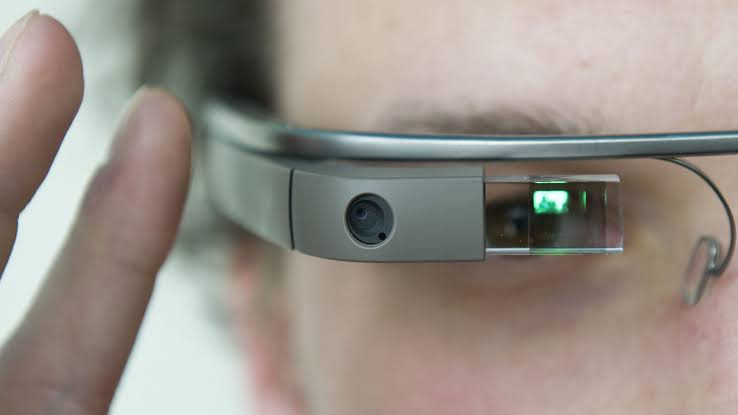
\includegraphics[width=0.85\textwidth]{pics/glass.jpg}
}

\section{Seguretat del hardware: necessitat i guerra comercial}

\frame{
  \frametitle{Introducció}
  Texto de ejemplo.
}

\subsection{Seguretat tècnica}

\frame{
  \frametitle{Seguretat tècnica (I)}
  Texto de ejemplo.
}

\frame{
  \frametitle{Seguretat tècnica (II)}
  Texto de ejemplo.
}

\subsection{Guerra comercial}

\frame{
  \frametitle{Guerra comercial (I)}
  Texto de ejemplo.
}

\frame{
  \frametitle{Guerra comercial (II)}
  Texto de ejemplo.
}

\subsection{El paper del hardware lliure}

\frame{
  \frametitle{El paper del hardware lliure}
  Texto de ejemplo.
}

\frame{
  \frametitle{Límits i matissos}
  Texto de ejemplo.
}

\frame{
  \frametitle{Conclusió}
  Texto de ejemplo.
}

\end{document}
